% Source: graduate-coursework/Sp26/CSCE775/course_notes/mc_prediction_guide.tex
% Description: Side-by-side comparison. Cells highlighted in \textcolor{Rose

\documentclass[border=4pt]{standalone}
\usepackage{amsfonts}
\usepackage{amsmath}
\usepackage{amssymb}
\usepackage{amsthm}
\usepackage[T1]{fontenc}
\usepackage{graphicx}
\usepackage{tikz}
\usepackage{xcolor}
\usetikzlibrary{arrows.meta, positioning, shapes.geometric, calc, decorations.pathreplacing}

\definecolor{Garnet}{HTML}{73000a}
\definecolor{SecondaryBlue}{HTML}{466A9F}
\definecolor{SecondaryGreen}{HTML}{65780B}
\definecolor{FlatRed}{HTML}{CC2E40}
\definecolor{FlatDark}{HTML}{1F414D}
\definecolor{FlatYellow}{HTML}{CED318}
\definecolor{FlatGold}{HTML}{A49137}
\definecolor{LightGray}{HTML}{F0F0F0}
\definecolor{Rose}{HTML}{CC2E40}

\renewcommand{\baselinestretch}{1.2}
\newcommand{\vocab}[1]{\textbf{\textcolor{Garnet}{#1}}}
\newcommand{\mathhighlight}[1]{\textcolor{SecondaryBlue}{#1}}

\begin{document}
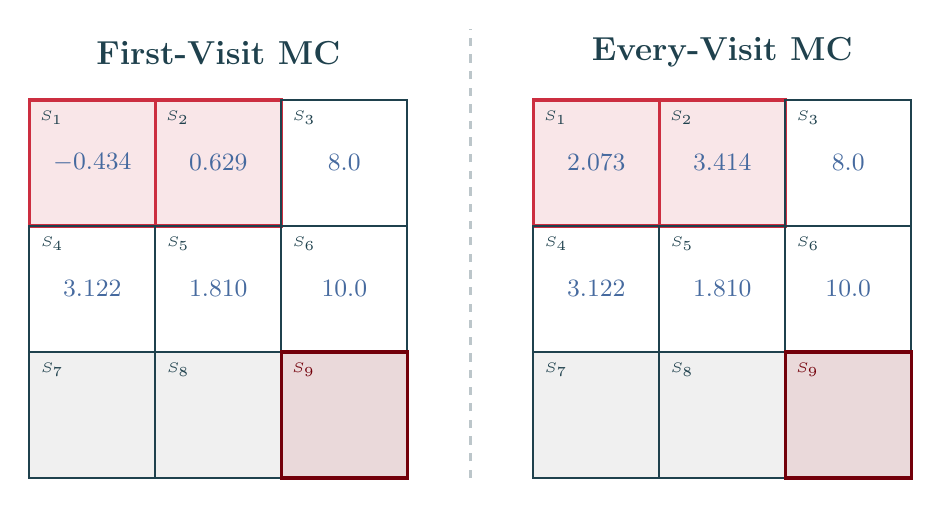
\begin{tikzpicture}[
    cell/.style={minimum size=1.6cm, draw=FlatDark, thick, font=\normalsize},
    diff/.style={cell, fill=Rose!12, draw=Rose, line width=1.2pt},
    goal/.style={cell, fill=Garnet!15, draw=Garnet, line width=1.2pt},
    empty/.style={cell, fill=LightGray},
    val/.style={font=\small\bfseries, SecondaryBlue},
    slabel/.style={font=\tiny, FlatDark},
    heading/.style={font=\large\bfseries, FlatDark}
]

% === First-Visit Grid (left) ===
\node[heading] at (1.6, 6.2) {First-Visit MC};

% Row 1
\node[diff] (fv1) at (0, 4.8) {};
\node[slabel, anchor=north west] at ([shift={(1pt,-1pt)}]fv1.north west) {$S_1$};
\node[val] at (fv1.center) {$-0.434$};

\node[diff] (fv2) at (1.6, 4.8) {};
\node[slabel, anchor=north west] at ([shift={(1pt,-1pt)}]fv2.north west) {$S_2$};
\node[val] at (fv2.center) {$0.629$};

\node[cell] (fv3) at (3.2, 4.8) {};
\node[slabel, anchor=north west] at ([shift={(1pt,-1pt)}]fv3.north west) {$S_3$};
\node[val] at (fv3.center) {$8.0$};

% Row 2
\node[cell] (fv4) at (0, 3.2) {};
\node[slabel, anchor=north west] at ([shift={(1pt,-1pt)}]fv4.north west) {$S_4$};
\node[val] at (fv4.center) {$3.122$};

\node[cell] (fv5) at (1.6, 3.2) {};
\node[slabel, anchor=north west] at ([shift={(1pt,-1pt)}]fv5.north west) {$S_5$};
\node[val] at (fv5.center) {$1.810$};

\node[cell] (fv6) at (3.2, 3.2) {};
\node[slabel, anchor=north west] at ([shift={(1pt,-1pt)}]fv6.north west) {$S_6$};
\node[val] at (fv6.center) {$10.0$};

% Row 3
\node[empty] (fv7) at (0, 1.6) {};
\node[slabel, anchor=north west] at ([shift={(1pt,-1pt)}]fv7.north west) {$S_7$};

\node[empty] (fv8) at (1.6, 1.6) {};
\node[slabel, anchor=north west] at ([shift={(1pt,-1pt)}]fv8.north west) {$S_8$};

\node[goal] (fv9) at (3.2, 1.6) {};
\node[slabel, anchor=north west] at ([shift={(1pt,-1pt)}]fv9.north west) {\textcolor{Garnet}{$S_9$}};

% === Every-Visit Grid (right) ===
\node[heading] at (8.0, 6.2) {Every-Visit MC};

% Row 1
\node[diff] (ev1) at (6.4, 4.8) {};
\node[slabel, anchor=north west] at ([shift={(1pt,-1pt)}]ev1.north west) {$S_1$};
\node[val] at (ev1.center) {$2.073$};

\node[diff] (ev2) at (8.0, 4.8) {};
\node[slabel, anchor=north west] at ([shift={(1pt,-1pt)}]ev2.north west) {$S_2$};
\node[val] at (ev2.center) {$3.414$};

\node[cell] (ev3) at (9.6, 4.8) {};
\node[slabel, anchor=north west] at ([shift={(1pt,-1pt)}]ev3.north west) {$S_3$};
\node[val] at (ev3.center) {$8.0$};

% Row 2
\node[cell] (ev4) at (6.4, 3.2) {};
\node[slabel, anchor=north west] at ([shift={(1pt,-1pt)}]ev4.north west) {$S_4$};
\node[val] at (ev4.center) {$3.122$};

\node[cell] (ev5) at (8.0, 3.2) {};
\node[slabel, anchor=north west] at ([shift={(1pt,-1pt)}]ev5.north west) {$S_5$};
\node[val] at (ev5.center) {$1.810$};

\node[cell] (ev6) at (9.6, 3.2) {};
\node[slabel, anchor=north west] at ([shift={(1pt,-1pt)}]ev6.north west) {$S_6$};
\node[val] at (ev6.center) {$10.0$};

% Row 3
\node[empty] (ev7) at (6.4, 1.6) {};
\node[slabel, anchor=north west] at ([shift={(1pt,-1pt)}]ev7.north west) {$S_7$};

\node[empty] (ev8) at (8.0, 1.6) {};
\node[slabel, anchor=north west] at ([shift={(1pt,-1pt)}]ev8.north west) {$S_8$};

\node[goal] (ev9) at (9.6, 1.6) {};
\node[slabel, anchor=north west] at ([shift={(1pt,-1pt)}]ev9.north west) {\textcolor{Garnet}{$S_9$}};

% Separator
\draw[FlatDark!30, dashed, line width=1pt] (4.8, 0.8) -- (4.8, 6.5);
\end{tikzpicture}
\end{document}
